\documentclass[12pt]{article}
\usepackage{geometry}
\geometry{a4paper}

\usepackage[parfill]{parskip}    % Activate to begin paragraphs with an empty line rather than an indent
\usepackage{graphicx}
\usepackage{amssymb}
\usepackage{epstopdf}
\usepackage{fancyhdr}
\usepackage{fullpage}
\usepackage{appendix}
\usepackage{newclude}
\usepackage{datetime}
\usepackage{hyperref}
\usepackage{color}
\usepackage{multicol}
\usepackage{tabularx}
\usepackage{enumerate}
\usepackage{enumitem}
\usepackage{listings}
\usepackage{wallpaper}
\usepackage{lastpage}
\usepackage{titling}
\usepackage{multind}
\usepackage[table]{xcolor}
\usepackage{mathtools}
\usepackage{tikz}
\usepackage{longtable}
\usepackage[section]{placeins}
%\geometry{landscape}
\usetikzlibrary{shapes,arrows}

\tikzstyle{block} = [rectangle, draw, text width = 6em, text centered, rounded corners, minimum height = 4em]
\tikzstyle{inputblock} = [rectangle, draw, text width = 24em, minimum height = 2.5em]
\tikzstyle{autographblock} = [rectangle, draw, fill = black!1, text height = 0, text depth = 2cm,text width = 24em, minimum height = 8em]
\tikzstyle{cloud} = [ellipse, draw, minimum height = 4em]
\tikzstyle{line} = [draw, -latex']

\makeindex{modules}


\newcommand{\usemodule}[1]{\index{modules}{#1}\texttt{#1}}

\definecolor{gray}{rgb}{0.5,0.5,0.5}
\definecolor{tableheader}{rgb}{0.7,0.7,0.7}

\setlist[description]{style=nextline}
\renewcommand{\familydefault}{\sfdefault}

% link setup
\hypersetup{
    colorlinks,
    citecolor=black,
    filecolor=black,
    linkcolor=black,
    urlcolor=black,
}

\DeclareGraphicsRule{.tif}{png}{.png}{`convert #1 `dirname #1`/`basename #1 .tif`.png}

% usefull commands:
\newcommand{\seeref}[1]{\ref{#1} p.\pageref{#1}}
%\newcommand{\see}[1]{ (zie \ref{#1} p.\pageref{#1})}
\newcommand{\seesee}[2]{ (zie \ref{#1} p.\pageref{#1},  \ref{#2} p.\pageref{#2})}

% style for code blocks
\lstset{
    linewidth=1\textwidth,
    breaklines=true,
    numbers=left,                   % where to put the line-numbers
    numberstyle=\tiny\color{gray},  % the style that is used for the line-numbers
    stepnumber=1,                   % the step between two line-numbers. If it's 1, each line 
    numbersep=5pt, 
    basicstyle=\footnotesize,
}

% Header and Footer settings
\URCornerWallPaper{0.13}{img/dop/koptekstlogo.png}
\pagestyle{fancy}
\fancyhead{}
\renewcommand{\headrulewidth}{0pt}

% Settings for table of contents.   
\setcounter{secnumdepth}{4}
\setcounter{tocdepth}{3}

\makeatletter
% some extra spacing for the table of contents
\renewcommand{\l@subsection}{\@dottedtocline{2}{1.5em}{3em}}
\renewcommand{\l@subsubsection}{\@dottedtocline{2}{2.7em}{4em}}

\renewcommand\paragraph{%
   \@startsection{paragraph}{4}{0mm}%
      {-\baselineskip}%
      {.5\baselineskip}%
      {\normalfont\normalsize\bfseries}}
\makeatother

\renewcommand{\dateseparator}{-}
\renewcommand{\figurename}{Figuur}

% Define variables
\newcommand{\customer}{Dimpact}
\newcommand{\projectname}{Dimpact}
\newcommand{\thecustomer}{\customer }
\newcommand{\customerdomain}{dimpact.nl}
\newcommand{\customerdomainfull}{http://www.dimpact.nl}
\newcommand{\customerdomainuc}{Dimpact.nl}
\newcommand{\authors}{David van Dijk \\ & Patrick Kraaij }
\newcommand{\version}{0.1}

\fancyfoot[L]{Functioneel ontwerp - \customer}
\fancyfoot[C]{v\version \ \ddmmyyyydate \today}
\fancyfoot[R]{\textbf{\thepage}\ / \pageref{LastPage}}

\title{\textbf{\customerdomainuc} \\ Functioneel Ontwerp}
\pretitle{\begin{flushleft}\LARGE}
\posttitle{\par\end{flushleft}}

\author{}  % skippen we voor maketitle
\date{}

% The actual Document:
\begin{document}
\ThisLRCornerWallPaper{0.8}{img/dop/voorbladlogo.png}

  \maketitle
 \vspace{-2.6cm}
  \begin{flushright}
\begin{tabularx}{4.6cm}{ X }
Dutch Open Projects         \\
Doornseweg 12                   \\  
3832 RL Leusden                 \\
T: +31[0]33 - 4 50 50 50        \\
F: +31[0]33 - 4 50 50 57        
\\*
\\*
\\*
\\*
\\*
\\*
\\*
\\*
\\*
\\*
\\*
\\*
\\*
\\*
\\*
\\*
\\*
\\*
\\*
\\*



\footnotesize
\copyright All rights reserved.         \\*
\footnotesize
No part of the contents of this publication may be reproduced, stored in a data processing system or transmitted in any form or by any means without the written permission of Dutch Open Projects B.V.

\end{tabularx}
\end{flushright}

\begin{tabularx}{\linewidth}{ p{3cm} X }
  Plaats & Leusden                                \\
  Laatst bijgewerkt & \ddmmyyyydate \today        \\
  Auteurs & \authors                          \\
  Versie & \version                                    \\
\end{tabularx}
\pagebreak




\pagebreak
\subsection*{Akkoord}
Voor akkoord:\\ \\
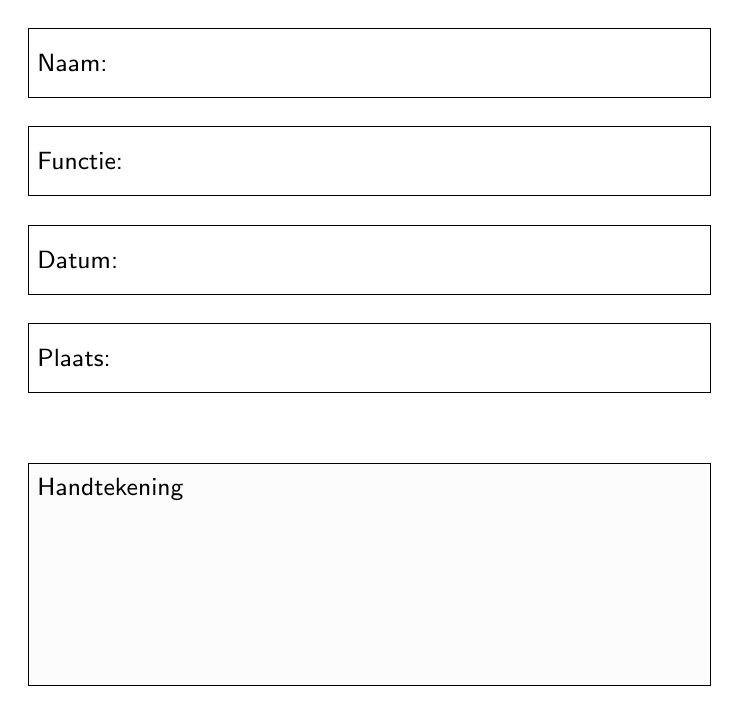
\begin{tikzpicture}
\tikzstyle{every node}=[font=\small];
\node [inputblock] (names) {Naam:};
\node [inputblock, below of = names, node distance = 1.25cm] (function) {Functie:};
\node [inputblock, below of = function, node distance = 1.25cm] (dates) {Datum:};
\node [inputblock, below of = dates, node distance = 1.25cm] (place) {Plaats:};
\node [autographblock, below of = place, node distance = 2.75cm] (autograph) {Handtekening};
\end{tikzpicture}
\pagebreak

% table of contents
\renewcommand*\contentsname{Inhoudsopgave}
\tableofcontents

\pagebreak


\section{Introductie}

\subsection{Management summary}
In het document Technisch Ontwerp \customerdomain \ wordt de technische implementatie beschreven. Het is een blauwdruk voor ontwikkelaars. 

\subsection{Opbouw document}
Dit document dient als leidraad voor de bouw van dit project. Het belangrijkste onderdeel ervan zijn daarom de componenten\seeone{componenten}. Componenten bieden een opsplitsing van de functionaliteiten binnen de website, zowel zichtbaar als niet zichtbaar. Tijdens de bouw zal een ontwikkelaar aan \'{e}\'{e}n specifiek component tegelijk werken. Daarnaast worden in dit document een aantal randzaken zoals deployment\seeone{deployment} en performance\seeone{performance} en algemene eisen\seeone{algemeen} beschreven in eerdere hoofdstukken. In de appendix vindt met een overzicht van Drupal specifieke zaken zoals content types en views, maar ook referentietabellen die aangeven waar welk onderdeel uit het interactieontwerp\seeone{ioto} of de design briefing\seeone{dbto} is beschreven.

\section{Pagina's}
\label{sec:paginas}

Hieronder worden alle pagina's opgesomd die zijn gemaakt in het wireframe. Per pagina worden alle blokken opgesomd. De volgende componenten komen voor op alle pagina's.
\begin{itemize}
  \item Logo en naam zie \ref{sec:logoennaam}
  \item Meta menu \ref{sec:metamenu}
  \item Tabs \ref{sec:tabspagina}
  \item Hoofdnavigatie \ref{sec:hoofdnavigatie}
  \item Zoekveld \ref{sec:zoekveld}
  \item Alfabetische balk \ref{sec:alfabetischebalk}
  \item Vrije HTML Footer \ref{sec:vrijehtmlfooter}
  \item DigiD \ref{sec:digid}
\end{itemize}

\subsection{Regios}
\label{sec:regios}

\begin{center}
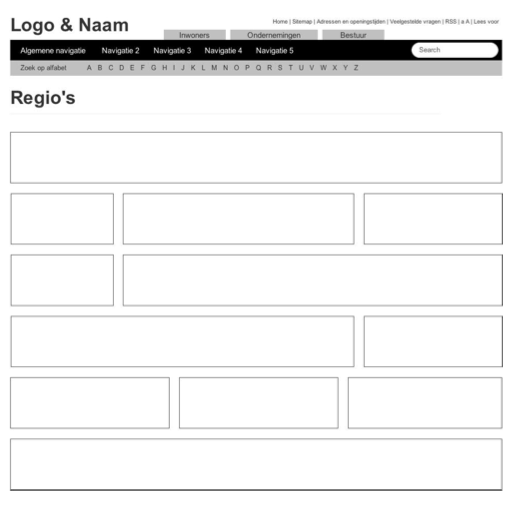
\includegraphics[scale=.5]{img/regions.png}
\end{center}

Op de pagina zijn de volgende regio's gedefinieerd. Aan de boven- en onderkant van de pagina zijn regio's over de hele breedte van de pagina beschikbaar. Daarnaast kent de template de volgende opstellingen.

\begin{description}
\item[Drie kolommen - smal / breed / smal] Deze opzet bestaat uit drie regio's waarbij de linker en rechter smaller zijn dan de middelste regio.
\item[Twee kolommen - smal / breed] Deze opzet bestaat uit twee regio's waarbij de linker regio smaller is dan de rechter.
\item[Twee kolommen - breed / smal] Deze opzet bestaat uit twee regio's waarbij de linker regio breder is dan de rechter.
\item[Drie kolommen] Deze opzet bestaat uit drie regio's die allen even breed zijn.
\end{description}

\subsection{Voorpagina}\label{voorpagina}

\subsubsection{Grid}

De template van de website bestaat uit een grid, een soort geraamte. Het grid is opgebouwd uit verschillende regio's. In elke regio kunnen blokken geplaatst worden. In de paragraaf \emph{Felix}\seeone{felix} staat beschreven hoe en welke je blokken kunt toevoegen aan een regio. 

\bigskip

\begin{center}
	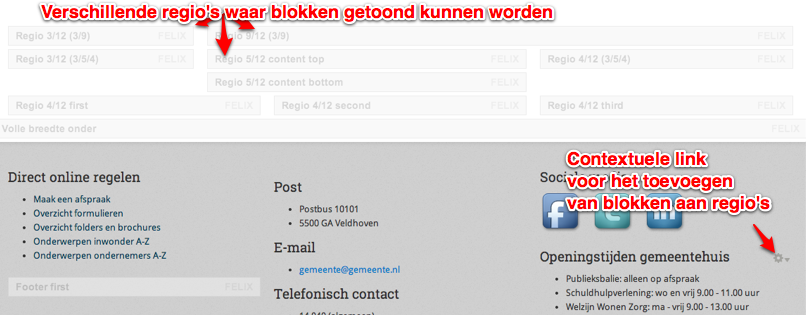
\includegraphics[width=\textwidth]{img/grid1.png}
\end{center}

\subsubsection{Blokken}

In het onderstaande afbeelding worden alle bestaande blokken op voorpagina in het kort toegelicht.

\bigskip

\begin{center}
	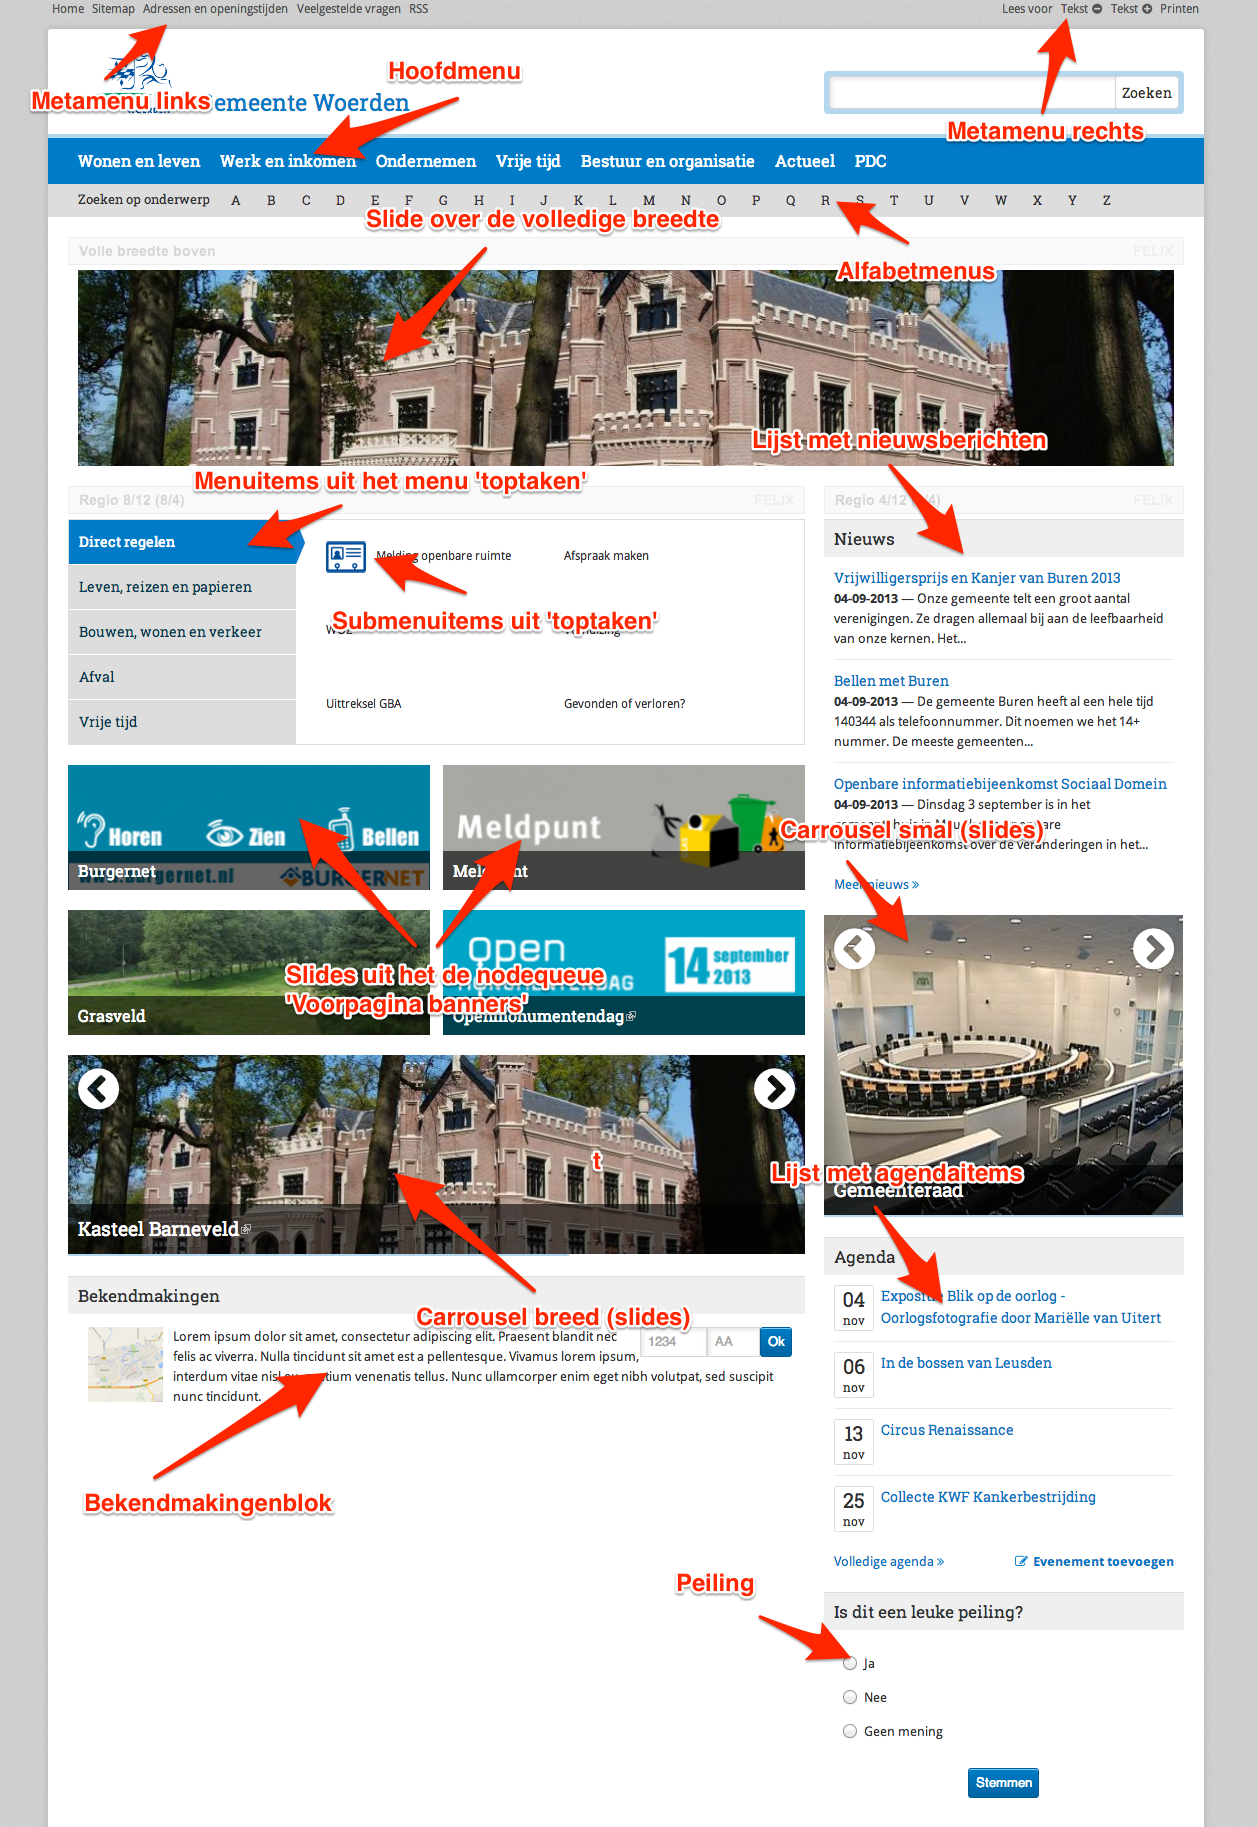
\includegraphics[width=\textwidth]{img/voorpagina.png}
\end{center}

\subsubsection{Footer}

In het onderstaande afbeelding worden alle bestaande blokken in de footer in het kort toegelicht. De footer bestaat uit 3 regio's waar blokken in gezet kunnen worden. De standaard configuratie is links een menu blok "Direct online regelen", in het hoofdstuk \emph{Menu}\seeone{menu} wordt beschreven hoe het menu te bewerken is. In de middenkolom staat blok met redactionele content. In de rechterkolom staan twee blokken; het eerste blok is het Dominion social blok. In paragraaf \emph{Social media}\seeone{socialmedia} staat beschreven hoe deze opties te beheren zijn. Daaronder staat nog een blok met redactionele content. Naast de standaard geconfigureerde blokken zijn in de drie regio's ook nog Felix blokken te zetten. 

\bigskip

\begin{center}
	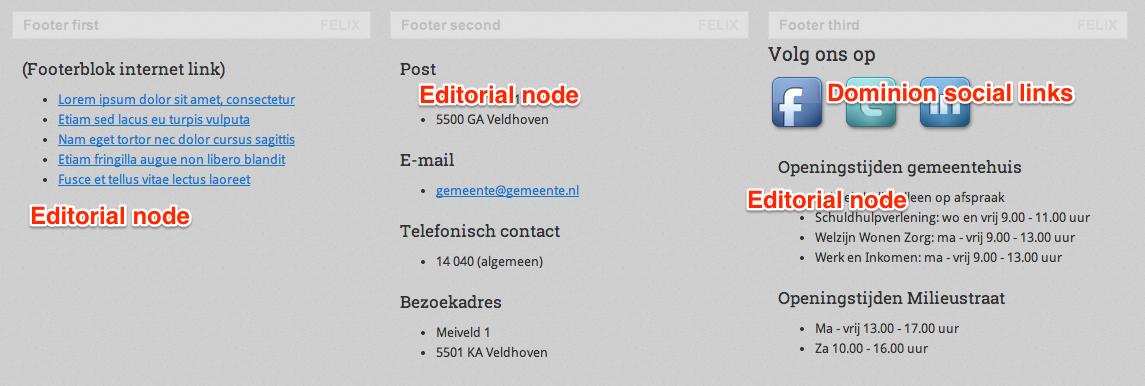
\includegraphics[width=\textwidth]{img/voorpagina3.png}
\end{center}
\subsection{Sub homepagina}
\label{sec:subhomepagina}
\subsection{Lijstpagina}
\label{sec:lijstpagina}
\subsection{Detail- en infopagina}
\label{sec:detaileninfopagina}

\begin{itemize}
  \item Agendalijstblok zie \ref{sec:agendalijst}
  \item Menublok hierarchisch zie \ref{sec:menublokhierarchisch}
  \item Gerelateerde items blok zie \ref{sec:gerelateerdeitems}
\end{itemize}

\subsubsection{Tabs}
\label{sec:detaileninfopaginatabs}

\begin{itemize}
  \item Agendalijstblok zie \ref{sec:agendalijst}
  \item Menublok hierarchisch zie \ref{sec:menublokhierarchisch}
  \item Gerelateerde items blok zie \ref{sec:gerelateerdeitems}
\end{itemize}

\subsection{Zoekresultaten}
\label{sec:zoekresultaten}
\subsection{Bekendmakingen}\label{bekendmakingen}

Bekendmakingen worden opgeslagen als Drupal nodes. Deze worden ge\"{i}mporteerd uit GVOP.

\subsubsection{Kaart en lijstweergave}\label{bekendmakingen-op-de-kaart}

De kaart wordt ontwikkeld m.b.v. views. Zie \seeref{bekendmakingen-markers}. De tekstuele resultaten worden middels een attachment bij deze view ingeladen \seeref{bekendmakingen-overzicht}.

De kaart wordt gemaakt met de \usemodule{gmap} module i.c.m. \usemodule{views}. Via \emph{exposed filters} wordt de volgende filtering aangeboden (in een apart blok):
\begin{itemize}
\item Zoeken op titel
\item Datum (van / tot)
\item Postcode (alleen exacte matching)
\item Status aanvraag (taxonomie, via checkboxes)
\end{itemize}
De filtering heeft zowel invloed op de kaart als op de lijst onder de kaart.


\subsection{Agenda}
\label{sec:agenda}

\begin{itemize}
  \item Tabsblok met nieuws en agenda zie \ref{sec:tabsmetnieuwsenagenda}
  \item Menublok hierarchisch zie \ref{sec:menublokhierarchisch}
  \item Gerelateerde items blok zie \ref{sec:gerelateerdeitems}
  \item Google Maps blok zie \ref{sec:maps}  
\end{itemize}

\subsection{Pagina met inhoudsopgave}
\label{sec:paginametinhoudsopgave}

\begin{itemize}
  \item Agendalijstblok zie \ref{sec:agendalijst}
  \item Menublok hierarchisch zie \ref{sec:menublokhierarchisch}
  \item Gerelateerde items blok zie \ref{sec:gerelateerdeitems}
  \item Downloadsblok zie \ref{sec:downloads}
\end{itemize}

\subsection{Smoelenboek}
\label{sec:smoelenboek}

\begin{itemize}
  \item Tabsblok met nieuws en agenda zie \ref{sec:tabsmetnieuwsenagenda}
  \item Grafisch element blok zie \ref{sec:grafischelement}
\end{itemize}
\subsection{Formulier}
\label{sec:formulier}
\subsection{Standaardpagina}
\label{sec:standaardpagina}

\begin{itemize}
  \item Nieuwslijstblok zie \ref{sec:nieuwslijst}
  \item Agendalijstblok zie \ref{sec:agendalijst}
  \item Grafisch element blok zie \ref{sec:grafischelement}
  \item Menublok hierarchisch zie \ref{sec:menublokhierarchisch}
  \item Content carrouselblok zie \ref{sec:contentcarrousel}
\end{itemize}



\end{document}
